%\normaltrue \difficilefalse \tdifficilefalse
%\correctionfalse
%
%%\UPSTIidClasse{11} % 11 sup, 12 spé
%%\newcommand{\UPSTIidClasse}{11}
%
%\exer{Vérin$\star$ \label{B2:07:500}}
\setcounter{question}{0}%\UPSTIcompetence[2]{B2-07}
%\index{Compétence B2-07}
%\index{Schéma-blocs}
%
%\ifcorrection
%\else
%\textbf{Pas de corrigé pour cet exercice.}
%\fi
%
%
%\ifprof 
%\else
%
%
% \fi
% 
%\question{}
%\ifprof
%\else 
%\fi
%
%
%%\question{Réaliser le schéma-blocs.}
%%\ifprof
%%\begin{figure}[H]
%%\centering
%%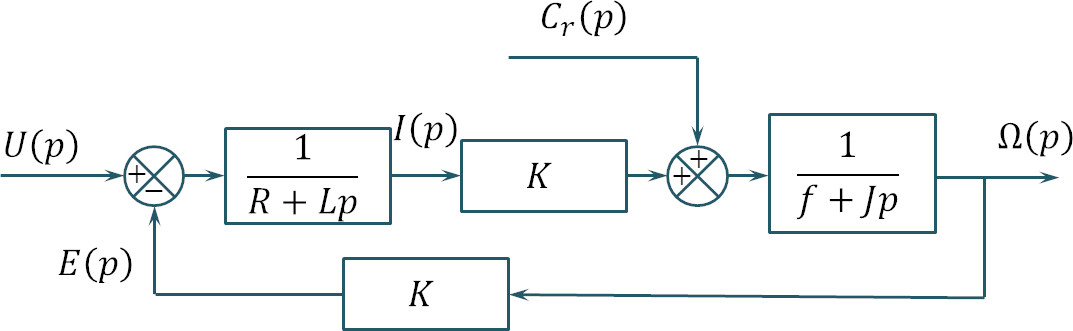
\includegraphics[width=\linewidth]{51_01_c}
%%%\caption{Évolution du couple utile en fonction de la vitesse de rotation pour des
%%%fréquences de commande de \SI{90}{Hz} à \SI{110}{Hz}. \label{fig_50_04}}
%%\end{figure}
%%\else
%%\fi
%
%
% 
%
%\ifprof
%\else
%\begin{flushright}
%\footnotesize{Corrigé  voir \ref{B2:07:500}.}
%\end{flushright}%
%\fi